% !TeX spellcheck = de_DE


\chapter{Einleitung}
	Die Veranstaltung "Data Mining und Maschinelles Lernen" behandelt, ebenso wie diese Zusammenfassung, den Teilbereich des maschinellen Lernens der künstlichen Intelligenz. Dabei werden Algorithmen entwickelt, durch die ein Computer sich selbstständig verbessert. Ein Teilgebiet dieses maschinellen Lernens ist das \emph{tiefe Lernen} (DL, für \emph{Deep Learning}), bei dem tiefe künstliche neuronale Netzwerke genutzt werden (dies wird im \autoref{c:deepLearning} näher behandelt). Dieser Zusammenhang ist in \autoref{fig:aiMlDl} dargestellt.

	Diese Zusammenfassung wird in die folgenden Bereiche einführen: k-Nächste Nachbarn, Lineare Modelle und Funktionsapproximation, Modellselektion und Evaluierung, Entscheidungsbäume, Ensemble-Methoden, Naive Bayes und Bayes-Netzwerke, die Stützvektormethode, Clusteranalyse und Assoziationsregeln und (Tiefe) Neuronale Netzwerke. Viele andere Bereiche werden allerdings auch nicht abgedeckt, \bspw Variational Learning, Details des Deep Learning, Gaussian Processes, Graphische Modelle, Kausalität, \dots Diese Inhalte sind zu Teilen in den Zusammenfassungen für die Kurse "Statistical Machine Learning", "Probabilistic Graphical Models" (noch nicht verfügbar, voraussichtlich im Wintersemester 2021/22), "Statistical Relational AI" (noch nicht verfügbar, voraussichtlich im Wintersemester 2021/22) sowie "Deep Learning: Architectures and Methods" (bald verfügbar) zu finden.

	\begin{figure}
		\centering
		\begin{tikzpicture}[align = center]
			\node (dl) {Tiefes \\ Lernen};
			\node [right = 1 of dl] (ml) {Maschinelles \\ Lernen};
			\node [right = 1 of ml] (ai) {Künstliche Intelligenz};

			\path (dl) -- coordinate(needle) (ml);

			\node [draw, ellipse, minimum height = 1.5cm, minimum width = 2cm] at (dl) {};
			\node [draw, ellipse, minimum height = 3cm, minimum width = 7cm] at (needle) {};
			\node [draw, ellipse, minimum height = 5cm, minimum width = 13cm] at (ml) {};
		\end{tikzpicture}
		\caption{Zusammenhang von künstlicher Intelligenz, maschinellem Lernen und tiefem Lernen.}
		\label{fig:aiMlDl}
	\end{figure}

	\section{Geschichte}
		Im Gegensatz zu den meisten Vermutungen hat die künstliche Intelligenz bereits eine lange Vergangenheit:
		\begin{description}[leftmargin = 2cm]
			\item[1950er] Geburt der künstlichen Intelligenz
			\item[1960er] Ära der Perzeptrons
			\item[1970er] Erster KI-Winter
			\item[1980er] Ära der Expertensysteme
			\item[1990er] Zweiter KI-Winter
			\item[2000er] Ära des statistischen maschinellen Lernens
			\item[2000er] Ära des tiefen Lernens
		\end{description}
		Das Perzeptron, welches im folgenden Abschnitt vorgestellt wird, hat die ersten großen Ergebnisse in der KI-Forschung produziert. Es hat zwar eine sehr mächtige Vorhersagekraft, es gibt jedoch Probleme, die nicht mit einem Perzeptron lösbar sind (Minsky, 1969). Diese Tatsache hat anschließend zu dem ersten KI-Winter geführt, in dem wenig geforscht wurde und das öffentliche Interesse abgeebbt ist. Gefolgt ist die Ära der Expertensysteme, Fall- und Regal-basierte KI-Systeme, die durch einen Menschen und logisches Schlussfolgern erstellt wurden. Jedoch haben auch diese Systeme zu viel versprochen und das öffentliche Interesse ist schnell abgeebbt.

		Nun betrat das moderne maschinelle Lernen mit dem \emph{statistischen} maschinellen Lernen das Feld, welches durch komplizierte statistische Modelle angetrieben und motiviert wurde. Die Ergebnisse haben sehr viele Erfolge gebracht, es gab jedoch kein großes Pressecho. Dies könnte unter anderem daher kommen, dass der Grundsatz der Forschung quantitative und messbare Ergebnisse waren und keine großen Ansprüche zur "Intelligenz" gestellt wurden. Darauf folgte die Ära des tiefen Lernens, also neuronale Netzwerke mit "vielen" Schichten, welches ein große Aufmerksamkeit von der Presse und Politik bekommt.

		\subsection{Das Perzeptron}
			Das von Frank Rosenblatt entwickelte \emph{Perzeptron} war das erste Modell, welches durch das menschliche Gehirn motiviert war, ein künstliches neuronales Netzwerk. Dabei werden viele kleine und einfache Einheiten (Neuronen) zu einem größeren Modell verbunden und das Lernen findet durch Anpassung der Verbindungsstärken (Synapsen) und -gewichten statt. Eine Darstellung eines solchen Perzeptrons ist in \autoref{fig:perceptron} gegeben. Dabei werden die Eingaben in der Neuronenschicht gewichtet und die Neuronen \emph{feuern}. Diese Ausgabe wird anschließend an das Ausgabeneuron weitergegeben, welches die \emph{Aktivierungen} akkumuliert und, sofern der akkumulierte Wert über einen gewissen Schwellenwert liegt, feuert. So kann eine binäre Klassifikation durchgeführt werden.

			Zum trainieren eines Perzeptrons werden bekannte Daten verwendet, in das Perzeptron eingegeben und die vorhergesagten Ergebnisse mit den echten verglichen. War die Vorhersage korrekt, wird nicht geändert. War die Vorhersage jedoch falsch, so werden die Verbindungsstärken so geändert, dass das Richtige vorhergesagt wird. Dies wird so lange wiederholt, bis keine Fehler mehr gemacht werden.

			Mit dem Wechsel zu tiefem Lernen werden diese einschichtigen nicht mehr verwendet, sondern es werden mehrere Neuronenschichten verwendet, die aufeinander Aufbauen (in \autoref{fig:mlp} in ein solches Netzwerk gezeigt). Neben der Nachteile des höheren Speicherverbrauchs, mehr benötigter Rechenkraft und der Anforderung an mehr Daten haben solche Modelle den großen Vorteil, dass sie eine deutlich höhere Vorhersagekraft besitzen.

			\begin{figure}
				\centering
				\begin{tikzpicture}[->]
					\node [input neuron] (a) {};
					\node [input neuron, below = 0.1 of a] (b) {};
					\node [input neuron, below = 0.1 of b] (c) {};
					\node [input neuron, below = 0.1 of c] (d) {};
					\node [input neuron, below = 0.1 of d] (e) {};

					\node [left = 2 of c] (I) {Input};

					\node [output neuron, right = 2 of c] (o) {};
					\node [right = 1 of o] (O) {Output};

					\draw (a) to[bend left = 10] (o);
					\draw (b) to[bend left = 5] (o);
					\draw (c) to (o);
					\draw (d) to[bend right = 5] (o);
					\draw (e) to[bend right = 10] (o);

					\draw (I) to[bend left = 10] (a);
					\draw (I) to[bend left = 5] (b);
					\draw (I) to (c);
					\draw (I) to[bend right = 5] (d);
					\draw (I) to[bend right = 10] (e);

					\draw (o) to (O);
				\end{tikzpicture}
				\caption{Darstellung eines einschichtigen Perzeptrons.}
				\label{fig:perceptron}
			\end{figure}

			\begin{figure}
				\centering
				\begin{tikzpicture}
					\node [input neuron] (a) {};
					\node [input neuron, below = 0.1 of a] (b) {};
					\node [input neuron, below = 0.1 of b] (c) {};
					\node [input neuron, below = 0.1 of c] (d) {};
					\node [input neuron, below = 0.1 of d] (e) {};

					\node [neuron, right = 1.5 of a] (l11) {};
					\node [neuron, right = 1.5 of b] (l12) {};
					\node [neuron, right = 1.5 of c] (l13) {};
					\node [neuron, right = 1.5 of d] (l14) {};
					\node [neuron, right = 1.5 of e] (l15) {};

					\node [neuron, right = 1.5 of l11] (l21) {};
					\node [neuron, right = 1.5 of l12] (l22) {};
					\node [neuron, right = 1.5 of l13] (l23) {};
					\node [neuron, right = 1.5 of l14] (l24) {};
					\node [neuron, right = 1.5 of l15] (l25) {};

					\node [neuron, right = 1.5 of l21] (l31) {};
					\node [neuron, right = 1.5 of l22] (l32) {};
					\node [neuron, right = 1.5 of l23] (l33) {};
					\node [neuron, right = 1.5 of l24] (l34) {};
					\node [neuron, right = 1.5 of l25] (l35) {};

					\node [output neuron, right = 1 of l33] (o) {};

					\draw (l31) to (o);
					\draw (l32) to (o);
					\draw (l33) to (o);
					\draw (l34) to (o);
					\draw (l35) to (o);

					\draw (a) to (l11);
					\draw (a) to (l12);
					\draw (a) to (l13);
					\draw (a) to (l14);
					\draw (a) to (l15);
					\draw (b) to (l11);
					\draw (b) to (l12);
					\draw (b) to (l13);
					\draw (b) to (l14);
					\draw (b) to (l15);
					\draw (c) to (l11);
					\draw (c) to (l12);
					\draw (c) to (l13);
					\draw (c) to (l14);
					\draw (c) to (l15);
					\draw (d) to (l11);
					\draw (d) to (l12);
					\draw (d) to (l13);
					\draw (d) to (l14);
					\draw (d) to (l15);
					\draw (e) to (l11);
					\draw (e) to (l12);
					\draw (e) to (l13);
					\draw (e) to (l14);
					\draw (e) to (l15);

					\draw (l11) to (l21);
					\draw (l11) to (l22);
					\draw (l11) to (l23);
					\draw (l11) to (l24);
					\draw (l11) to (l25);
					\draw (l12) to (l21);
					\draw (l12) to (l22);
					\draw (l12) to (l23);
					\draw (l12) to (l24);
					\draw (l12) to (l25);
					\draw (l13) to (l21);
					\draw (l13) to (l22);
					\draw (l13) to (l23);
					\draw (l13) to (l24);
					\draw (l13) to (l25);
					\draw (l14) to (l21);
					\draw (l14) to (l22);
					\draw (l14) to (l23);
					\draw (l14) to (l24);
					\draw (l14) to (l25);
					\draw (l15) to (l21);
					\draw (l15) to (l22);
					\draw (l15) to (l23);
					\draw (l15) to (l24);
					\draw (l15) to (l25);

					\draw (l21) to (l31);
					\draw (l21) to (l32);
					\draw (l21) to (l33);
					\draw (l21) to (l34);
					\draw (l21) to (l35);
					\draw (l22) to (l31);
					\draw (l22) to (l32);
					\draw (l22) to (l33);
					\draw (l22) to (l34);
					\draw (l22) to (l35);
					\draw (l23) to (l31);
					\draw (l23) to (l32);
					\draw (l23) to (l33);
					\draw (l23) to (l34);
					\draw (l23) to (l35);
					\draw (l24) to (l31);
					\draw (l24) to (l32);
					\draw (l24) to (l33);
					\draw (l24) to (l34);
					\draw (l24) to (l35);
					\draw (l25) to (l31);
					\draw (l25) to (l32);
					\draw (l25) to (l33);
					\draw (l25) to (l34);
					\draw (l25) to (l35);
				\end{tikzpicture}
				\caption{Darstellung eines mehrschichtigen Perzeptrons.}
				\label{fig:mlp}
			\end{figure}
		% end
	% end

	\section{KI Heute}
		Heute gibt es vier entscheidende Unterschiede zu vergangenen KI-Systemen:
		\begin{enumerate}
			\item Die Modelle sind größer.
				\begin{itemize}
					\item Früher wurden neuronale Netzwerke mit ein bis drei Schichten und hunderte bis tausende Neuronen verwendet.
					\item Heutige Modelle haben hunderte Schichten und hunderttausende Neuronen.
				\end{itemize}
			\item Es sind mehr Daten verfügbar.
				\begin{itemize}
					\item Früher waren tausende Bilder, hunderte Stunden Audiomaterial und hunderttausende Wörter verfügbar.
					\item Heute sind es Milliarden Bilder, Milliarden Stunden Audiomaterial und hunderte Milliarden Wörter.
					\item Diese Daten werden dabei in vielen großen Firmen gesammelt, \bspw hat YouTube mehr als zehn Milliarden Videos, Alibaba tätigt mehr als zwölf Milliarden Verkäufe pro Jahr, Facebook-Nutzer laden hunderte Milliarden Bilder pro Jahr hoch und Google kennt mehr als hundert Billionen Webseiten.
				\end{itemize}
			\item Heute Computer sind Leistungsfähiger.
				\begin{itemize}
					\item Früher konnte eine CPU \ca eine Millionen Operationen pro Sekunde ausführen und es gab keine GPUs.
					\item Heutige CPUs können mehr als eine Billionen Operationen pro Sekunde und heutige GPUs können mehr als zehn Billionen Operationen pro Sekunde ausführen.
				\end{itemize}
			\item Die Systeme funktionieren und lösen viele Aufgaben.
		\end{enumerate}
		Dabei ist der Hauptmotor der künstlichen Intelligenz aktuell das maschinelle Lernen.
	% end

	\section{Was ist Maschinelles Lernen?}
		\emph{Maschinelles Lernen} ist die Automatisierung von Automatisierung, es werden Teile des Computers so programmiert, dass sie sich anschließend selbstständig "programmieren". Das ist nötig, da das Schreiben von Software oftmals der Flaschenhals in der Entwicklung ist, da die Daten so schnell mehr werden. Es ist also klug, die Daten zu nutzen, um die Software selbst zu erstellen. Im Gegensatz zur traditionellen Programmierung werden also keine Ausgaben durch ein Programm erstellt, sondern es wird ein Programm aus Ausgaben erstellen (siehe \autoref{fig:traditionalVsMl}). Die Entwicklung von ML-Komponenten ist dabei ein Kreislauf, dargestellt in \autoref{fig:mlPipeline}.

		Anwendungsgebiete von maschinellem Lernen sind beispielsweise Websuche, Computational Biologie/Cognitive Science/Social Science/\dots, Finanzwelt, E-Commerce, Robotik, Debugging, Industrie 4.0 und viele mehr.

		\begin{figure}
			\centering
			\begin{subfigure}{0.49\linewidth}
				\centering
				\begin{tikzpicture}
					\node [draw, rectangle, minimum height = 1cm, minimum width = 2.5cm] (a) {Computer};
					\coordinate [above = 0.3 of a.west] (b);
					\coordinate [below = 0.3 of a.west] (c);
					\node [left = 0.75 of b] (d) {Daten};
					\node [left = 0.75 of c] (e) {Programm};
					\node [right = 0.75 of a.east] (f) {Ausgabe};
					\draw [->] (d) to (b);
					\draw [->] (e) to (c);
					\draw [->] (a.east) to (f);
				\end{tikzpicture}
				\caption{Traditionelle Programmierung}
			\end{subfigure}
			~
			\begin{subfigure}{0.49\linewidth}
				\centering
				\begin{tikzpicture}
					\node [draw, rectangle, minimum height = 1cm, minimum width = 2.5cm] (a) {Computer};
					\coordinate [above = 0.3 of a.west] (b);
					\coordinate [below = 0.3 of a.west] (c);
					\node [left = 0.75 of b] (d) {Daten};
					\node [left = 0.75 of c] (e) {Ausgabe};
					\node [right = 0.75 of a.east] (f) {Programm};
					\draw [->] (d) to (b);
					\draw [->] (e) to (c);
					\draw [->] (a.east) to (f);
				\end{tikzpicture}
				\caption{Maschinelles Lernen}
			\end{subfigure}
			\caption{Traditionelle Programmierung (links) im Vergleich zu maschinellem Lernen (rechts).}
			\label{fig:traditionalVsMl}
		\end{figure}

		\begin{figure}
			\centering
			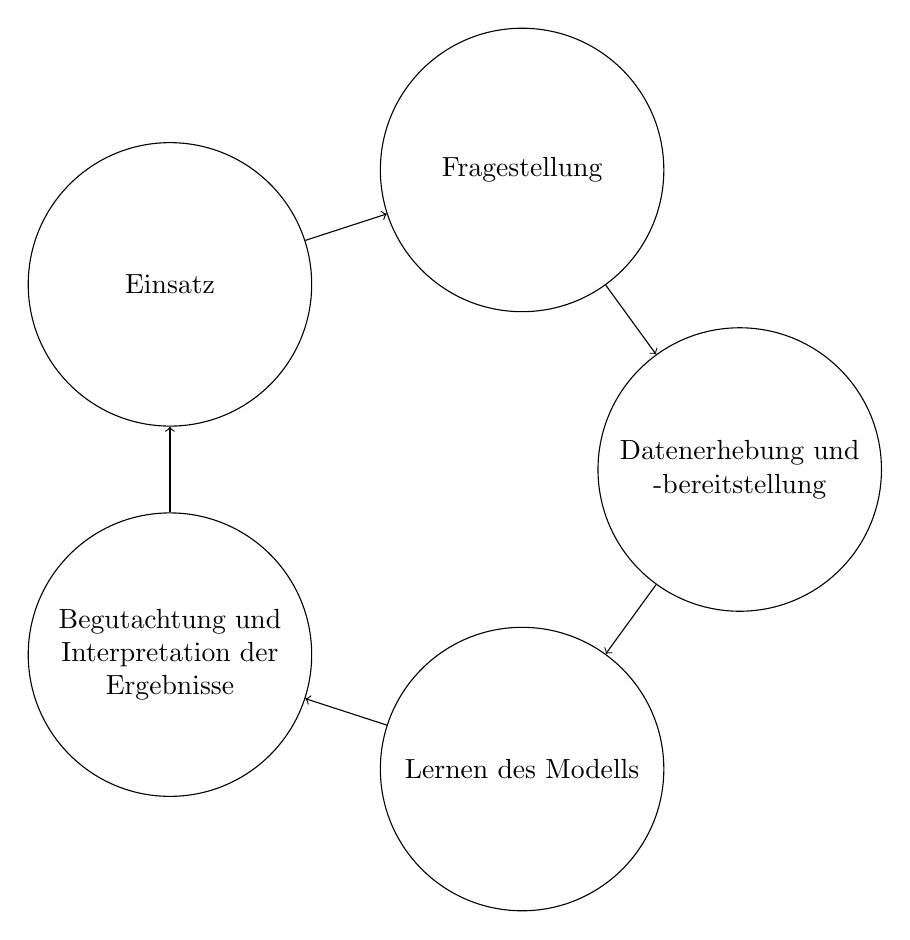
\begin{tikzpicture}[->, align = center, every node/.style = { draw, circle, minimum height = 2cm, minimum width = 3.6cm }]
				\node (a) at (-288:4cm) {Fragestellung};
				\node (b) at (-  0:4cm) {Datenerhebung und \\ -bereitstellung};
				\node (c) at (- 72:4cm) {Lernen des Modells};
				\node (d) at (-144:4cm) {Begutachtung und \\ Interpretation der \\ Ergebnisse};
				\node (e) at (-216:4cm) {Einsatz};
				\draw (a) to (b);
				\draw (b) to (c);
				\draw (c) to (d);
				\draw (d) to (e);
				\draw (e) to (a);
			\end{tikzpicture}
			\caption{Kreislauf der Erstellung von ML-Komponenten.}
			\label{fig:mlPipeline}
		\end{figure}

		\subsection{Kurzgefasst}
			Im Bereich des maschinellen Lernens gibt es viele tausende Algorithmen und hunderte neue Algorithmen pro Jahr. Dabei adressiert jeder Algorithmus die folgenden drei Fragestellungen:
			\begin{enumerate}
				\item Wie wird das Modell \emph{repräsentiert}? \\
					Entscheidungsbäume, Regeln/logische Programme, Instanzen, Probabilistische Graphische Modelle, Neuronale Netzwerke, Stützvektormaschinen, Ensembles, \dots
				\item Wie wird das Modell \emph{optimiert}? \\
					Kombinatorische Optimierung (\zB Greedy-Suche), Konvexe und nichtlineare Optimierung (\zB Gradientenabstieg), Optimierung unter Randbedingungen (\zB lineare Programmierung), \dots
				\item Wie wird das Modell \emph{evaluiert} und \emph{beurteilt}? \\
					Korrektklassifikationsrate (Accuracy), Genauigkeit (Precision) und Trefferquote (Recall), Quadrierter Fehler, Likelihood, A-Posteriori Wahrscheinlichkeit, Kosten/Nutzen, Margin, Entropie, KL-Divergenz, \dots
			\end{enumerate}

			Dabei gibt es vier große Kategorien des maschinellen Lernens:
			\begin{description}
				\item[Überwacht (Induktiv)] Die Trainingsdaten erhalten neben Eingaben auch gewünschten Ausgaben. \\
					Englisch: \emph{Supervised Learning}
				\item[Unüberwacht] Die Trainingsdaten erhalten nur Eingaben und \emph{keine} Ausgaben. \\
					Englisch: \emph{Unsupervised Learning}
				\item[Teilweise Überwacht] Die Trainingsdaten \emph{einige} gewünschte Ausgaben, aber nicht alle. \\
					Englisch: \emph{Semi-supervised Learning}
				\item[Verstärkend] Der Algorithmus wird belohnt nachdem er eine Reihe an Aktionen ausgeführt hat und die Belohnung wird maximiert. \\
					Englisch: \emph{Reinforcement Learning}
			\end{description}
			Die Bereiche des überwachten und unüberwachten Lernens lassen sich dann noch weiter einordnen, was in \autoref{fig:mlTypes} gezeigt ist.

			\begin{figure}
				\centering
				\begin{tikzpicture}[
							->,
							align = center,
							block/.style = {
								draw,
								rectangle,
								minimum width = 3.25cm,
								minimum height = 1.5cm,
							},
								small/.style = {
								minimum height = 0.8cm,
							},
						]
					\node [block] (ml) {Maschinelles \\ Lernen};
					\node [block, right = 2 of ml, yshift = +3cm] (supervised) {Überwachtes \\ Lernen};
					\node [block, right = 2 of ml] (unsupervised) {Unüberwachtes \\ Lernen};
					\node [block, right = 2 of ml, yshift = -3cm] (rl) {Verstärkendes \\ Lernen};

					\node [block, small, right = 2 of supervised, yshift = +0.75cm] (class) {Klassifikation};
					\node [block, small, right = 2 of supervised, yshift = -0.75cm] (regress) {Regression};

					\node [block, small, right = 2 of unsupervised, yshift = +0.75cm] (dimred) {Dim.-Reduktion};
					\node [block, small, right = 2 of unsupervised, yshift = -0.75cm] (cluster) {Clustering};

					\draw (ml.east) to [bend right, out = -45+10, in = +180-45] (supervised.west);
					\draw (ml.east) to (unsupervised.west);
					\draw (ml.east) to [bend left,  out = +45-10, in = -180+45] (rl.west);

					\draw (supervised.east) to [bend right, out = -45+30, in = +180-45+30] (class.west);
					\draw (supervised.east) to [bend left,  out = +45-30, in = -180+45-30] (regress.west);

					\draw (unsupervised.east) to [bend right, out = -45+30, in = +180-45+30] (dimred.west);
					\draw (unsupervised.east) to [bend left,  out = +45-30, in = -180+45-30] (cluster.west);
				\end{tikzpicture}
				\caption{Arten des maschinellen Lernens.}
				\label{fig:mlTypes}
			\end{figure}
		% end
	% end
% end

\chapter{Grundlagen} % N/A
	\todo{Content}

	\section{CRISP: Verlaufsmodell der Wissensentdeckung} % 2.25, 2.26
		\todo{Content}
	% end

	\section{Klassifikation und Regression} % 2.31, 2.32, 2.33, 2.34
		\todo{Content}
	% end

	\section{Statistik} % N/A
		\todo{Content}

		\subsection{Erwartungswert, 2.24, 3.12, 3.13} % 2.49, 2.50, 2.51, 2.52
			\todo{Content}
		% end

		\subsection{Bias} % 2.53, 2.54
			\todo{Content}
		% end

		\subsection{Normalverteilung} % 3.6
			\todo{Content}
		% end

		\subsection{Bayes-Statistik} % 3.14
			\todo{Content}
		% end

		\subsection{Bedingte Wahrscheinlichkeiten} % 4.11
			\todo{Content}
		% end

		\subsection{Konfidenzintervalle} % 4.26
			\todo{Content}
		% end
	% end
% end

\chapter{k-Nächste Nachbarn (kNN)} % 2.2, 2.3, 2.7, 2.8, 2.9
	\todo{Content}

	\section{Globale und Lokale Modelle} % 2.2
		\todo{Content}
	% end

	\section{Beispiel} % 2.4, 2.5
		\todo{Content}
	% end

	\section{Ähnlichkeitsmaße} % 2.6, 2.10, 2.11
		\todo{Content}
	% end

	\section{Auswahlfunktion} % 2.12
		\todo{Content}
	% end

	\section{Überanpassung} % 2.13, 2.14
		\todo{Content}
	% end

	\section{Asymptotische Ergebnisse und Fluch der hohen Dimension} % 2.15, 2.16, 2.17
		\todo{Content}
	% end
% end

\chapter{Lineare Modelle und Funktionsapproximation} % 2.63, 3.2, 3.3, 3.4, 3.24
	\todo{Content}

	\section{Lineare Modelle} % 2.28, 2.30, 2.37, 2.38, 2.39, 2.47
		\todo{Content}

		\subsection{Modell-Anpassung} % 2.42, 2.43, 2.44, 2.45, 2.46
			\todo{Content}
		% end
	% end

	\section{Fehler} % 2.48, 2.55, 2.56
		\todo{Content}

		\subsection{Bias und Varianz} % 2.57, 2.58, 2.59, 2.60
			\todo{Content}
		% end
	% end

	\section{Gütekriterien} % N/A
		\todo{Content}

		\subsection{Maximum Likelihood} % 3.5
			\todo{Content}

			\subsubsection{Maximum Likelihood für Lineare Modelle} % 3.7, 3.8
				\todo{Content}
			% end
		% end

		\subsection{Kreuzentropie} % 3.9
			\todo{Content}
		% end
	% end

	\section{Fluch der hohen Dimension} % 2.61
		\todo{Content}
	% end

	\section{Logistische Regression} % 3.36, 3.37
		\todo{Content}
	% end
% end

\chapter{Modellselektion und Evaluierung} % 2.18, 2.19, 2.20, 3.1, 3.2, 3.10, 3.11
	\todo{Content}

	\section{Aufteilung in Test- und Trainingsmenge} % 2.21, 2.22, 2.23
		\todo{Content}

		\subsection{Kreuzvalidierung} % 2.24, 3.12, 3.13
			\todo{Content}
		% end
	% end

	\section{Bayes'sche Modellselektion} % 3.15
		\todo{Content}

		\subsection{Approximation der A-Posteriori Wahrscheinlichkeit} % 3.16
			\todo{Content}
		% end

		\subsection{Bayes Information Criterion (BIC)} % 3.17, 3.18
			\todo{Content}
		% end

		\subsection{Minimum Description Length (MDL)} % 3.19, 3.20, 3.21, 3.22
			\todo{Content}
		% end

		\subsection{Zusammenhang zwischen BIC und MDL} % 3.23
			\todo{Content}
		% end
	% end

	\section{Evaluierungsmaße} % 3.25, 3.26, 3.27, 3.28
		\todo{Content}

		\subsection{ROC-Analyse und -Kurve} % 3.38, 3.39, 3.40, 3.41, 3.42
			\todo{Content}
		% end

		\subsection{Präzision und Recall} % 3.43, 3.44
			\todo{Content}
		% end

		\subsection{F-Measure, Breakeven Point} % 3.45
			\todo{Content}
		% end
	% end

	\section{Zusammenfassung von Experimentellen Ergebnissen} % 3.29, 3.30
		\todo{Content}

		\subsection{Vorzeichen-Test} % 3.31, 3.32, 3.33, 3.34
			\todo{Content}
		% end
	% end
% end

\chapter{Baumbasierte Verfahren} % 4.1, 4.2, 4.3, 4.4, 4.5, 4.6, 4.7, 4.45
	\todo{Content}

	\section{Information und Informationsgewinn} % 4.12
		\todo{Content}

		\subsection{Numerische Werte} % 4.15
			\todo{Content}
		% end
	% end

	\section{Top-Down Induction of Decision Trees (TDIDT): ID3} % 4.21, 4.22
		\todo{Content}
	% end

	\section{Stutzen (Pruning) des Baumes} % 4.23, 4.24, 4.25
		\todo{Content}

		\subsection{Fehlerschätzung} % 4.27, 4.28, 4.29, 4.30, 4.31
			\todo{Content}
		% end

		\subsection{Anwendung zum Stutzen} % 4.32
			\todo{Content}
		% end
	% end

	\section{Andere Gütemaße} % N/A
		\todo{Content}

		\subsection{Gini-Index} % 4.33, 4.34
			\todo{Content}
		% end

		\subsection{Regression} % 4.35
			\todo{Content}
		% end
	% end

	\section{Evaluierung} % 4.36, 4.37, 4.38
		\todo{Content}

		\subsection{Fehlergewichtung} % 4.39
			\todo{Content}
		% end
	% end
% end

\chapter{Ensemble-Methoden} % 5.1, 5.2, 5.3, 5.4, 5.52
	\todo{Content}

	\section{Zufallswälder (Random Forests)} % 5.5, 5.6, 5.7, 5.8, 5.9, 5.10, 5.11, 5.12, 5.13, 5.14
		\todo{Content}
	% end

	\section{Bagging} % 5.22, 5.23
		\todo{Content}
	% end

	\section{Boosting} % 5.25, 5.26, 5.27, 5.28, 5.29, 5.35, 5.38, 5.39
		\todo{Content}

		\subsection{AdaBoost} % 5.30, 5.31, 5.32, 5.33, 5.34
			\todo{Content}
		% end
	% end

	\section{Vergleich} % 5.40
		\todo{Content}
	% end

	\section{Gradient Boosting} % 5.41, 5.42, 5.43, 5.44, 5.45, 5.46
		\todo{Content}
	% end
% end

\chapter{Probabilistische Graphische Modelle und Stützvektormethode} % 6.1, 6.23, 6.34
	\todo{Content}

	\section{Naive Bayes Klassifikator} % 6.2, 6.13, 6.15, 6.16, 6.17, 6.18, 6.19, 6.20, 6.21, 6.22
		\todo{Content}

		\subsection{Beispiel} % 6.3, 6.4, 6.5, 6.6, 6.7, 6.8, 6.9, 6.10, 6.11, 6.14
			\todo{Content}
		% end
	% end

	\section{Bayes'sche Netzwerke} % 6.24, 6.25, 6.26, 6.27, 6.28
		\todo{Content}
	% end

	\section{Parameterschätzung bei Vollständigen Daten: Maximum Likelihood} % 6.29, 6.30
		\todo{Content}
	% end

	\section{Parameterschätzung bei Unvollständigen Daten: Expectation Maximization (EM)} % 6.31, 6.32, 6.33
		\todo{Content}
	% end

	\section{Diskriminative Ansätze} % 6.35, 6.36, 6.37, 6.40
		\todo{Content}

		\subsection{Stützvektormethode} % 6.42, 6.43, 6.44, 6.45, 6.51, 6.52, 6.62
			\todo{Content}

			\subsubsection{Optimalität der Hyperebene} % 6.53, 6.54, 6.55, 6.56
				\todo{Content}
			% end

			\subsubsection{Optimierungsproblem} % 6.57, 6.58, 6.59, 6.60, 6.61, 6.63
				\todo{Content}
			% end
		% end

		\subsection{Nicht linear trennbare Daten} % 6.64, 6.65, 6.69
			\todo{Content}

			\subsubsection{Transformation in ein lineares Problem} % 6.66, 6.67
				\todo{Content}
			% end

			\subsubsection{Kernel-Trick} % 6.68
				\todo{Content}
			% end
		% end
	% end
% end

\chapter{Clustering} % 6.70, 6.71, 6.72, 6.81, 6.94
	\todo{Content}

	\section{Dendrogramme und Hierarchisches Clustering (Agglomerativ/Aufteilend)} % 6.73, 6.74, 6.75, 6.76, 6.77
		\todo{Content}
	% end

	\section{(Vorgetäuschte) Strukturen, Anzahl Cluster und Ausreißer} % 6.78, 6.79, 6.80
		\todo{Content}
	% end

	\section{Partitionierung und K-Means} % 6.83, 6.84, 6.89, 6.90, 6.91, 6.92, 6.93
		\todo{Content}
	% end
% end

\chapter{Deep Learning und Faltende Neuronale Netzwerke} % 7.1, 7.5, 7.6, 7.7, 7.67, 7.68, 7.69, 8.41
	\label{c:deepLearning}

	\todo{Content}

	\section{Modellierung eines Neurons} % 7.8, 7.12, 7.53
		\todo{Content}
	% end

	\section{Aufeinanderschichten von Einheiten} % 7.14
		\todo{Content}
	% end

	\section{Faltungsschichten} % 7.19, 7.20, 7.21, 7.22, 7.23, 7.24, 7.25, 7.26, 7.27, 7.49, 7.50
		\todo{Content}

		\subsection{Räumliche Auflösung, Stride und Zero-Padding} % 7.29, 7.30, 7.31, 7.32, 7.33, 7.34, 7.35, 7.36, 7.37, 7.38, 7.39, 7.40, 7.41, 7.42, 7.43, 7.44, 7.45, 7.46, 7.47, 7.48
			\todo{Content}
		% end
	% end

	\section{Räumliche Zusammenfassung} % 7.55, 7.56, 7.57
		\todo{Content}
	% end

	\section{Vollständig verbundene Schichten} % 7.59, 7.60, 7.61
		\todo{Content}
	% end

	\section{Training} % 8.7
		\todo{Content}

		\subsection{Stochastic Gradient Descent} % 7.12, 7.13, 7.15, 7.16, 7.17, 7.63, 8.9, 8.10, 8.21, 8.22
			\todo{Content}
		% end

		\subsection{Backpropagation} % 7.18, 8.11
			\todo{Content}

			\subsubsection{Sequential Brick} % 8.12
				\todo{Content}
			% end

			\subsubsection{Loss Bricks} % 8.13, 8.14
				\todo{Content}
			% end

			\subsubsection{Linear Brick} % 8.15
				\todo{Content}
			% end

			\subsubsection{Activation Function Bricks} % 8.16, 8.17
				\todo{Content}

				\paragraph{Subgradienten} % 8.18
					\todo{Content}
				% end

				\paragraph{Leaky ReLU} % 8.19
					\todo{Content}
				% end
			% end
		% end
	% end

	\section{Vermeidung von Überanpassung} % 8.23
		\todo{Content}

		\subsection{Dropout} % 8.24, 8.25, 8.26
			\todo{Content}
		% end

		\subsection{Datenaugmentierung} % 8.27
			\todo{Content}
		% end
	% end

	\section{Fine-Tuning und Transfer Learning} % 8.28, 8.29, 8.30
		\todo{Content}
	% end

	\section{Visualisierung} % 8.31, 8.32, 8.33, 8.34, 8.35, 8.36, 8.37, 8.38
		\todo{Content}

		\subsection{Täuschen von CNNs} % 8.39, 8.40
			\todo{Content}
		% end
	% end

	\section{Beispiele: LeNet-5, AlexNet, GoogLeNet} % 7.64, 7.65, 7.66, 8.2, 8.3, 8.4, 8.5, 8.6
		\todo{Content}
	% end
% end

\chapter{Data Mining: Apriori und PageRank} % 9.1, 9.2, 9.3, 9.18
	\todo{Content}

	\section{Assoziationsregeln} % 9.4, 9.5, 9.8, 9.9, 9.10
		\todo{Content}

		\subsection{Binäre Datenbanken} % 9.6, 9.7
			\todo{Content}
		% end
	% end

	\section{Apriori Algorithmus} % 9.11, 9.14, 9.15, 9.16, 9.17, 9.19
		\todo{Content}
	% end

	\section{Regelbewertung} % 9.20, 9.21, 9.22, 9.23
		\todo{Content}
	% end

	\section{Web Mining} % 9.24, 9.25
		\todo{Content}

		\subsection{Ranking von Webseiten} % 9.26
			\todo{Content}
		% end

		\subsection{PageRank} % 9.27, 9.28, 9.29, 9.30
			\todo{Content}
		% end
	% end
% end
